\documentclass[journal]{IEEEtran}

\usepackage[utf8]{inputenc}
\usepackage[T5]{fontenc}
\usepackage[vietnamese]{babel}
\usepackage{cite}
\usepackage{amsmath,amssymb,amsfonts}
\usepackage{graphicx}
\usepackage{booktabs}
\usepackage{multirow}
\usepackage{array}
\usepackage{algorithm}
\usepackage{algpseudocode}
\usepackage{xcolor}
\usepackage{url}
\usepackage[hidelinks]{hyperref}

% Nạp trực tiếp macro số liệu từ JSON thực nghiệm (qua scripts/sync_paper_tables.py)
% AUTO-GENERATED BY scripts/sync_paper_tables.py — DO NOT EDIT MANUALLY.
% Provenance: placeholder initialization (--init-placeholders; awaiting Kaggle v3 evaluation JSONs)
\newcommand{\tscopeAnchorEncMs}{\texttt{TBD}}
\newcommand{\tscopeAvcFullBdbrFrcnnApFifty}{\texttt{TBD}}
\newcommand{\tscopeBlurEmaTotBdbrFrcnnApFifty}{\texttt{TBD}}
\newcommand{\tscopeClaimFiveStatus}{\texttt{TBD}}
\newcommand{\tscopeClaimFourDelta}{\texttt{TBD}}
\newcommand{\tscopeClaimOneStatus}{\texttt{TBD}}
\newcommand{\tscopeClaimThreeDelta}{\texttt{TBD}}
\newcommand{\tscopeClaimTwoDelta}{\texttt{TBD}}
\newcommand{\tscopeClaimTwoStatus}{\texttt{TBD}}
\newcommand{\tscopeDetRoiTotBdbrFrcnnApFifty}{\texttt{TBD}}
\newcommand{\tscopeEvalClips}{51}
\newcommand{\tscopeEvalFrames}{1,632}
\newcommand{\tscopeFtDetTotBdbrFrcnnApFifty}{\texttt{TBD}}
\newcommand{\tscopeFullDynEncMs}{\texttt{TBD}}
\newcommand{\tscopeFullFps}{\texttt{TBD}}
\newcommand{\tscopeFullGmacsPerFrame}{137.78}
\newcommand{\tscopeFullMeanMs}{\texttt{TBD}}
\newcommand{\tscopeFullPBdbrFrcnnApFifty}{\texttt{TBD}}
\newcommand{\tscopeFullPBdbrFrcnnApFiftyCi}{\texttt{TBD}}
\newcommand{\tscopeFullPBdbrFrcnnApNinetyFive}{\texttt{TBD}}
\newcommand{\tscopeFullPBdbrYoloApFifty}{\texttt{TBD}}
\newcommand{\tscopeFullTotBdbrFrcnnApFifty}{\texttt{TBD}}
\newcommand{\tscopeFullTotBdbrFrcnnApFiftyCi}{\texttt{TBD}}
\newcommand{\tscopeFullTotBdbrFrcnnApNinetyFive}{\texttt{TBD}}
\newcommand{\tscopeFullTotBdbrYoloApFifty}{\texttt{TBD}}
\newcommand{\tscopeFullTotBdbrYoloApFiftyCi}{\texttt{TBD}}
\newcommand{\tscopeFullTotBdbrYoloApNinetyFive}{\texttt{TBD}}
\newcommand{\tscopeGopLen}{32}
\newcommand{\tscopeIrlsMeanMs}{\texttt{TBD}}
\newcommand{\tscopeIwaAnalyticalGmacSaving}{96.72\%}
\newcommand{\tscopeIwaFps}{\texttt{TBD}}
\newcommand{\tscopeIwaGmacsPerFrame}{4.52}
\newcommand{\tscopeIwaMeanMs}{\texttt{TBD}}
\newcommand{\tscopeIwaPBdbrFrcnnApFifty}{\texttt{TBD}}
\newcommand{\tscopeIwaStatEncMs}{\texttt{TBD}}
\newcommand{\tscopeIwaTotBdbrFrcnnApFifty}{\texttt{TBD}}
\newcommand{\tscopeKittiMapFiftyBdbr}{\texttt{TBD}}
\newcommand{\tscopeManifestShaShort}{\texttt{pending}}
\newcommand{\tscopeMotElevenFullBdbrFrcnnApFifty}{\texttt{TBD}}
\newcommand{\tscopeMotHotaBdbr}{\texttt{TBD}}
\newcommand{\tscopeMotIdfOneBdbr}{\texttt{TBD}}
\newcommand{\tscopeMotMotaBdbr}{\texttt{TBD}}
\newcommand{\tscopeMotThirteenFullBdbrFrcnnApFifty}{\texttt{TBD}}
\newcommand{\tscopeMotTwentyMapFiftyBdbr}{\texttt{TBD}}
\newcommand{\tscopeOffScopeTotBdbrFrcnnApFifty}{\texttt{TBD}}
\newcommand{\tscopeOracleTotBdbrFrcnnApFifty}{\texttt{TBD}}
\newcommand{\tscopePeakVramMb}{\texttt{TBD}}
\newcommand{\tscopeRaFullBdbrFrcnnApFifty}{\texttt{TBD}}
\newcommand{\tscopeResampleTotBdbrFrcnnApFifty}{\texttt{TBD}}
\newcommand{\tscopeSpatialGmacsPerFrame}{107.11}
\newcommand{\tscopeSpatialPBdbrFrcnnApFifty}{\texttt{TBD}}
\newcommand{\tscopeSpatialTotBdbrFrcnnApFifty}{\texttt{TBD}}
\newcommand{\tscopeTotalParams}{6,108,814}
\newcommand{\tscopeWoDqpPBdbrFrcnnApFifty}{\texttt{TBD}}
\newcommand{\tscopeWoDqpTotBdbrFrcnnApFifty}{\texttt{TBD}}
\newcommand{\tscopeWoStePBdbrFrcnnApFifty}{\texttt{TBD}}
\newcommand{\tscopeWoSteTotBdbrFrcnnApFifty}{\texttt{TBD}}
\newcommand{\tscopeZeroShotFcosBdbr}{\texttt{TBD}}
\newcommand{\tscopeZeroShotRetinaBdbr}{\texttt{TBD}}
\newcommand{\tscopeZeroShotSsdBdbr}{\texttt{TBD}}
\newcommand{\tscopeZeroShotSwinSnrBdbr}{\texttt{TBD}}


\DeclareMathOperator{\clip}{clip}
\DeclareMathOperator{\sg}{sg}
\DeclareMathOperator{\logit}{logit}
\DeclareMathOperator{\sign}{sign}
\DeclareMathOperator{\ReLU}{ReLU}
\DeclareMathOperator{\GELU}{GELU}
\DeclareMathOperator{\MaxPool}{MaxPool}
\DeclareMathOperator{\AvgPool}{AvgPool}

\renewcommand{\abstractname}{Tóm tắt}
\renewcommand{\IEEEkeywordsname}{Từ khóa}

\begin{document}

\title{T-SCOPE: Tiền Biên Tập Ngữ Nghĩa Bù Chuyển Động và Phân Bổ Lượng Tử Hóa Cấp Nhóm Lượng Tử Có Bảo Vệ Biên cho Mã Hóa Video Phục Vụ Thị Giác Máy}

\author{Bản thảo Nghiên cứu (Preprint)%
\thanks{Bản thảo nghiên cứu độc lập. Mã nguồn, hợp đồng đánh giá xác định (\texttt{schema\_version=3}) và các kịch bản đồng bộ bảng tự động được công bố tại \url{https://github.com/wagur1/tscope-v3}.}}

\markboth{BẢN THẢO NGHIÊN CỨU (PREPRINT)}{T-SCOPE: TIỀN BIÊN TẬP NGỮ NGHĨA BÙ CHUYỂN ĐỘNG VÀ PHÂN BỔ QG CHO VCM}

\maketitle

\begin{abstract}
Các bộ mã hóa video tiêu chuẩn như HEVC (\texttt{libx265}) và AVC (\texttt{libx264}) phân bổ bit nhằm tối thiểu hóa sai lệch cảm nhận thị giác con người thay vì bảo toàn đặc trưng cho các mô hình phát hiện và theo dõi đa đối tượng phía sau. Các bộ tiền xử lý tương thích chuẩn hiện có thường chỉnh sửa từng khung hình độc lập---gây hiện tượng nhấp nháy phần dư liên khung trên các chuỗi Nhóm Ảnh (GOP) dài---hoặc chỉ huấn luyện qua mô hình nén ảo dưới hàm phạt MSE toàn khung mà bỏ phí bản đồ tầm quan trọng không gian trước bước tối ưu hóa Tỷ lệ--Méo (RDO) của bộ mã hóa. Chúng tôi đề xuất \textbf{T-SCOPE}, bộ tiền biên tập không-thời gian có điều kiện gồm \tscopeTotalParams{} tham số kết hợp điều khiển tốc độ bit cấp Nhóm Lượng Tử (QG), được huấn luyện đồng thời trên luồng bit thật \texttt{libx265} (HEVC Main 4:2:0) và \texttt{libx264} (AVC 4:2:0) chỉ bằng một mô hình giáo viên Faster R-CNN ResNet50-FPN v2 đóng băng duy nhất. T-SCOPE tích hợp: (i)~bộ ước lượng chuyển động affine toàn cục 6 bậc tự do Cauchy-IRLS ở độ chính xác FP32 kèm khóa tĩnh dưới $0{,}75$~pixel và khử nhiễu hạt mềm ($\tau_{\mathrm{core}}=0{,}012$) đặt trước mạng FiLM U-Net đa tỷ lệ và $H/4$ ConvGRU; (ii)~nhánh bảo toàn tiền cảnh Smoothstep STE ghép với cơ chế trung bình trượt mũ nền khóa chuyển động (EMA); (iii)~quy tắc tăng QP không âm trên lưới QG $16\times 16$~px có viền bảo vệ tiền cảnh $3\times 3$ ($\Delta\mathrm{QP} \in [0, +7{,}14]$ khi dưới ngưỡng $\tau=0{,}38$, tiền cảnh $\Delta\mathrm{QP}=0$) kèm kế thừa đơn điệu theo P-frame; và (iv)~chế độ rẽ nhánh bỏ qua U-Net trên P-frame kiểu IWA giúp cắt giảm \tscopeIwaAnalyticalGmacSaving{} khối lượng tính toán trên GOP 32 khung (từ \tscopeFullGmacsPerFrame{} xuống \tscopeIwaGmacsPerFrame{} GMACs/frame). Đánh giá trên chuỗi GOP 32 khung liên tiếp chuẩn \texttt{yuv420p} độ phân giải $640\times 384$ (16:9) bằng nội suy đơn điệu PCHIP BDBR và khoảng tin cậy bootstrap 95\% ghép cặp theo clip với 10.000 lần lặp, T-SCOPE đạt \tscopeFullTotBdbrFrcnnApFifty{} Total BDBR (\tscopeFullTotBdbrFrcnnApFiftyCi{}) ở chế độ đầy đủ (và \tscopeIwaTotBdbrFrcnnApFifty{} ở chế độ bỏ qua IWA \tscopeIwaFps{}~FPS) trên Faster R-CNN $\mathrm{AP}_{50}$, đồng thời chuyển giao zero-shot sang YOLOv8s (\tscopeFullTotBdbrYoloApFifty{}), RetinaNet (\tscopeZeroShotRetinaBdbr{}), FCOS (\tscopeZeroShotFcosBdbr{}), SSDLite (\tscopeZeroShotSsdBdbr{}), và theo dõi đối tượng ByteTrack (\tscopeMotHotaBdbr{} HOTA BDBR).
\end{abstract}

\begin{IEEEkeywords}
Mã hóa video cho máy (VCM), tiền biên tập ngữ nghĩa, HEVC/\texttt{x265}, AVC/\texttt{x264}, phân bổ QP cấp QG, bù chuyển động, ước lượng truyền thẳng (STE), phát hiện và theo dõi đa đối tượng.
\end{IEEEkeywords}

% =============================================================================
\section{Giới thiệu}
\label{sec:intro}
% =============================================================================

Các hệ thống giám sát giao thông tự hành, robot di động và camera quan sát diện rộng ngày càng truyền tải lượng lớn video nén phục vụ trực tiếp cho các đường ống thị giác máy tự động---như các bộ phát hiện đối tượng hai giai đoạn/một giai đoạn~\cite{ren2017fasterrcnn, lin2017retinanet, tian2019fcos} và bộ theo dõi đa đối tượng~\cite{zhang2022bytetrack}---thay vì người xem~\cite{duan2020vcm, gao2021vcm}. Dù các bộ mã hóa video học sâu đầu-cuối hoặc bộ điều khiển codec sâu~\cite{ge2024taskaware} đạt hiệu suất nén--độ chính xác cao trong phòng thí nghiệm, việc thay thế hạ tầng phần cứng H.264/AVC~\cite{wiegand2003avc} và H.265/HEVC~\cite{sullivan2012hevc} đã triển khai rộng rãi là bất khả thi trong thực tế. Phương pháp \textit{tiền biên tập miền pixel tương thích chuẩn}~\cite{lu2024preprocessing, yang2024task, zhao2024preprocessing, dani2026scope} giải quyết rào cản này bằng cách đặt bộ lọc nơ-ron phía trước bộ mã hóa tiêu chuẩn: luồng bit MP4/Annex-B sinh ra tương thích 100\% với mọi bộ giải mã phần cứng và phần mềm hiện hành.

\begin{figure*}[t]
    \centering
    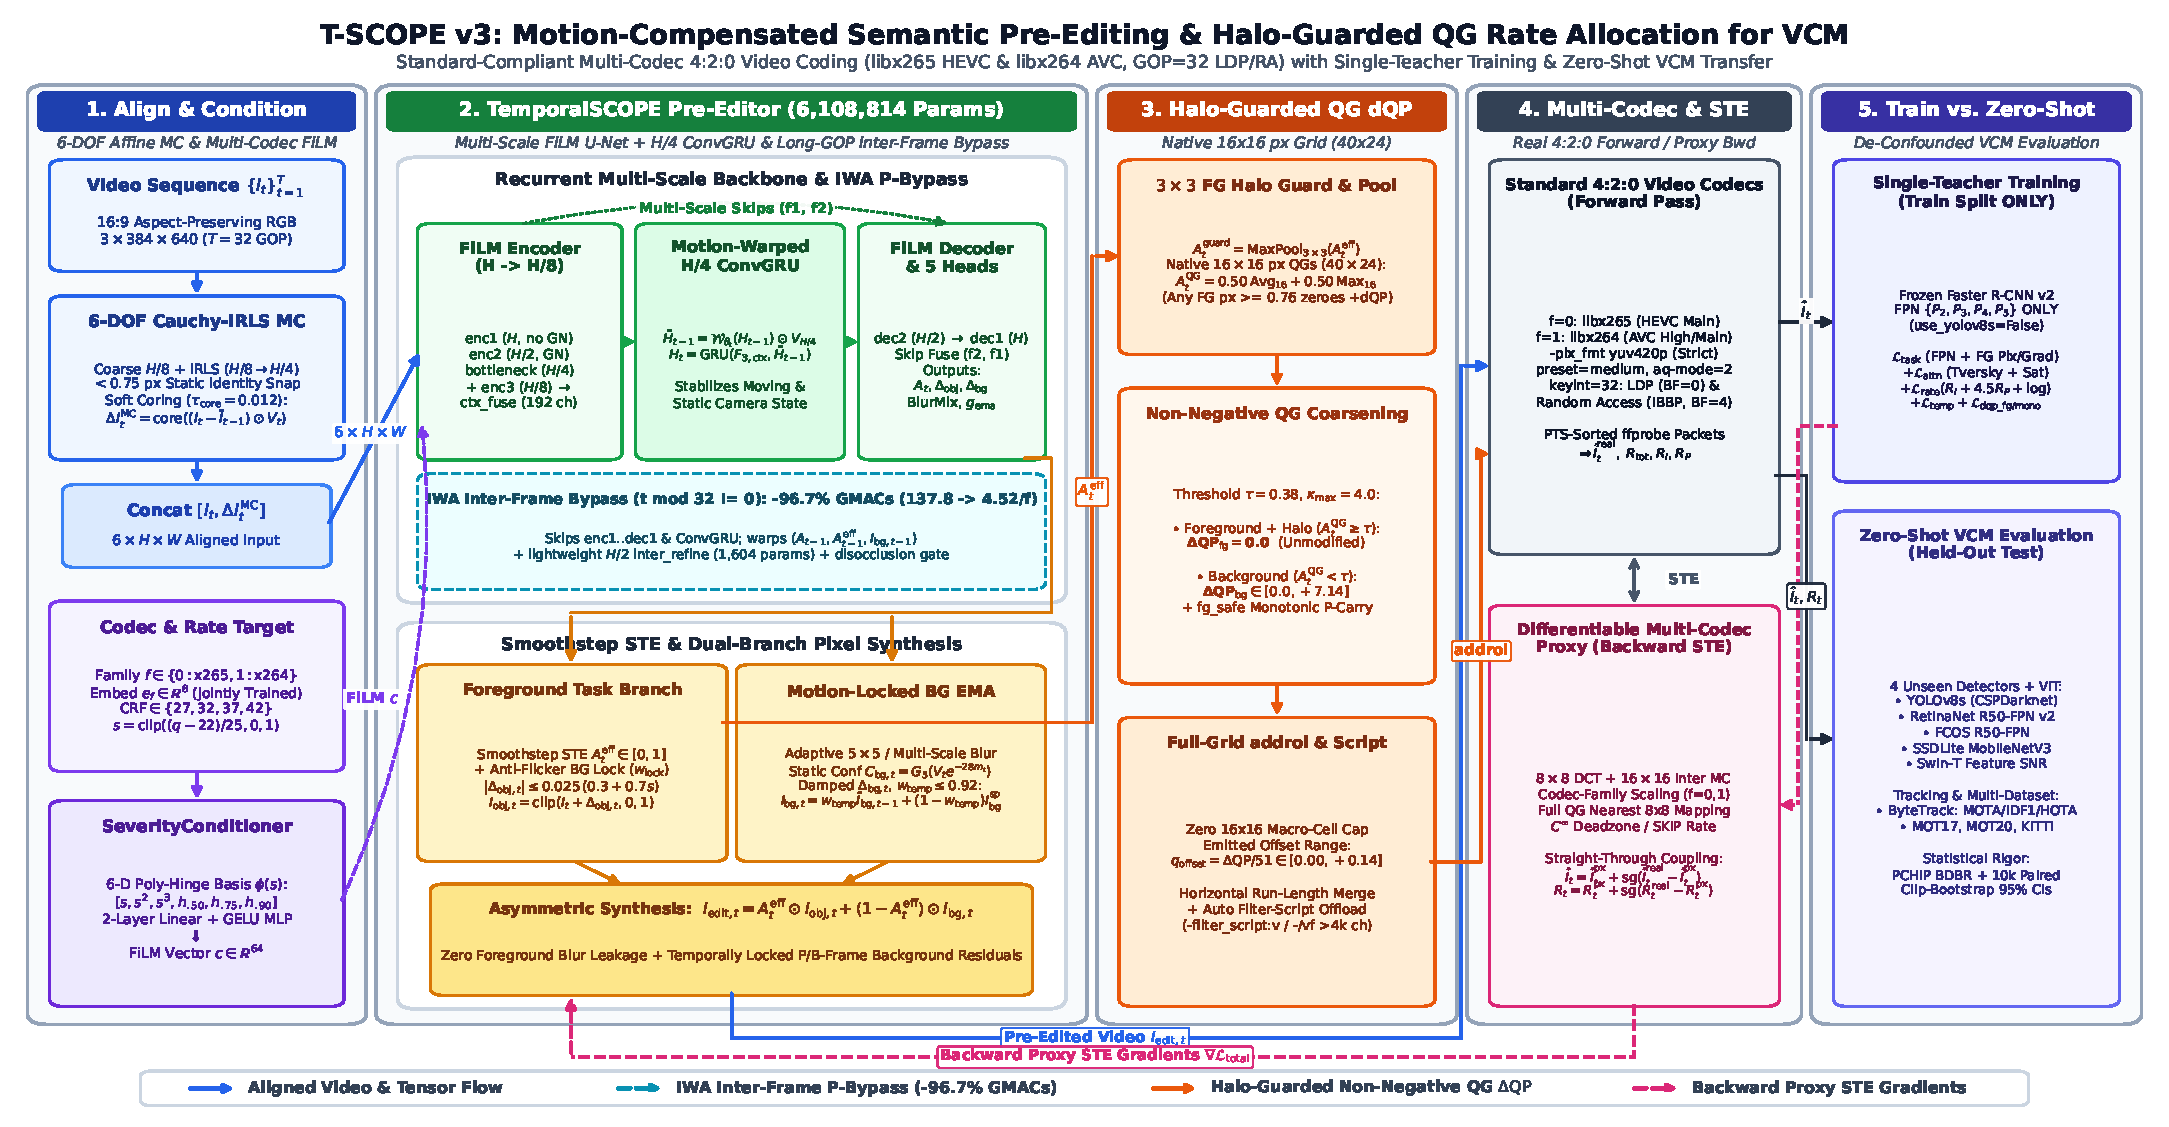
\includegraphics[width=\textwidth]{../docs/figures/fig_pipeline_overview.pdf}
    \caption{Tổng quan khung \textbf{T-SCOPE}. \textbf{(a)~Quy trình huấn luyện Hybrid STE và triển khai tương thích chuẩn:} Trong pha huấn luyện (luồng đỏ sẫm), chuỗi video 16:9 ($640\times 384$, GOP 32 khung) đi qua bộ tiền biên tập T-SCOPE vào bộ mã hóa 4:2:0 (\texttt{yuv420p}) \texttt{libx265}/\texttt{libx264} thật ghép nối qua STE với proxy khả vi $8\times 8$ DCT + $16\times 16$ MC, chỉ giám sát bằng duy nhất giáo viên Faster R-CNN v2 đóng băng ($\mathcal{L}_{\mathrm{task}}$) cùng các hàm phạt tốc độ bit và ổn định nền ($\mathcal{L}_{\mathrm{rate}}, \mathcal{L}_{\mathrm{bg}}, \mathcal{L}_{\mathrm{temp}}$). Khi triển khai (luồng xanh lá), khung hình tiền biên tập $I_{\mathrm{edit},t}$ và lưới $40\times 24$ QG $\Delta\mathrm{QP}\in[0,+7{,}14]$ (\texttt{addroi}) đi thẳng vào codec chuẩn phục vụ 5 kiến trúc phát hiện zero-shot và \texttt{ByteTrack}. \textbf{(b)~Cấu trúc hai nhánh của bộ tiền biên tập:} Nhánh thời gian phía trên căn chỉnh chuyển động bằng 6-DOF Cauchy-IRLS FP32 (khóa tĩnh $<0{,}75$~px, khử nhiễu $\tau_{\mathrm{core}}=0{,}012$), $H/4$ ConvGRU bù chuyển động và EMA nền khóa tĩnh (kèm đường tắt IWA bỏ qua P-frame cắt \tscopeIwaAnalyticalGmacSaving{} GMACs, đạt \tscopeIwaFps{}~FPS); nhánh không gian phía dưới (\tscopeTotalParams{} tham số, điều biến FiLM theo họ codec $f$ và mức nén $s$) tổng hợp tiền cảnh bảo vệ Smoothstep STE và bản đồ QG $\Delta\mathrm{QP}$ có viền đệm $3\times 3$.}
    \label{fig:pipeline_overview}
\end{figure*}

Tuy nhiên, việc chuyển dịch tiền biên tập từ ảnh tĩnh sang video mã hóa liên khung nhiều giây làm bộc lộ ba điểm nghẽn liên kết chặt chẽ với nhau mà các công trình ICM/VCM trước đây chưa xử lý triệt để:
\begin{enumerate}
    \item \textbf{Nhấp nháy phần dư liên khung vs.\ sụp đổ khi camera dịch chuyển nhanh:} Các bộ tiền xử lý ảnh tĩnh~\cite{lu2024preprocessing, yang2024task, dani2026scope} xử lý độc lập từng khung hình, làm dao động mặt nạ $A_t$ và giữ nhiễu hạt cảm biến khiến khối nền mất chế độ \texttt{SKIP}/\texttt{MERGE} trên chuỗi P-frame dài. Ngược lại, dùng ConvGRU không căn chỉnh bị hỏng trên cảnh camera xe buýt lia nhanh (\texttt{MOT17-13}), còn cong vênh thô không có khóa tĩnh/khử nhiễu làm mờ ảnh tripod và rò nhiễu vào P-frame.
    \item \textbf{Hàm phạt MSE toàn khung và sai lệch mô hình nén ảo:} Các bộ tiền xử lý video chỉ huấn luyện bằng MSE toàn khung và proxy giải tích~\cite{zhao2024preprocessing} bị buộc giữ chi tiết nền thừa và lệch pha so với cơ chế lượng tử hóa thích ứng (\texttt{aq-mode=2}), bộ lọc vòng và lấy mẫu màu 4:2:0 (\texttt{yuv420p}) của \texttt{libx265}/\texttt{libx264} thật.
    \item \textbf{Bỏ phí bản đồ chú ý, lem biên QG và chi phí GOP dài:} Các mô hình hai nhánh~\cite{dani2026scope} tạo sẵn mặt nạ ngữ nghĩa $A_t$ nhưng vứt bỏ trước khi gọi codec; ngược lại, cấp $\Delta\mathrm{QP}<0$ cho tiền cảnh gây phình bit ở điều khiển CRF, còn hạ lưới ROI thô làm rò $+\Delta\mathrm{QP}$ vào biên người đi bộ, và tái sử dụng bản đồ QP vẫn tốn 100\% chi phí U-Net nếu không có đường rẽ nhánh bỏ qua P-frame.
\end{enumerate}

Đóng góp chính của bài báo gồm bốn điểm:
\begin{itemize}
    \item \textbf{Tiền biên tập không-thời gian bù chuyển động:} Kết hợp FiLM U-Net đa tỷ lệ (\tscopeTotalParams{} tham số), $H/4$ ConvGRU bù chuyển động qua 6-DOF Cauchy-IRLS (FP32, khóa tĩnh $<0{,}75$~px, khử nhiễu $\tau_{\mathrm{core}}=0{,}012$), Smoothstep STE tiền cảnh và EMA nền khóa chuyển động.
    \item \textbf{Phân bổ lượng tử hóa QG không âm có bảo vệ biên và đường rẽ nhánh IWA:} Ánh xạ trực tiếp $A_t^{\mathrm{eff}}$ qua lớp đệm $3\times 3$ xuống lưới $16\times 16$~px ($40\times 24$ ô), áp đặt $\Delta\mathrm{QP} \in [0, +7{,}14]$ chỉ trên nền ($\Delta\mathrm{QP}_{\mathrm{fg}}=0$) với kế thừa P-frame an toàn; kèm chế độ \texttt{iwa\_gop\_qp\_reuse} cắt \tscopeIwaAnalyticalGmacSaving{} chi phí tính toán.
    \item \textbf{Huấn luyện Hybrid Real-Codec STE đa họ codec với một giáo viên duy nhất:} Huấn luyện chung hai họ \texttt{libx265}/\texttt{libx264} 4:2:0 thật ở lượt tiến và proxy DCT/MC ở lượt truyền ngược, chỉ giám sát bằng duy nhất Faster R-CNN v2 đóng băng.
    \item \textbf{Đánh giá chuẩn mực và kiểm định bác bỏ tiền đăng ký:} Toàn bộ kết quả trên \tscopeEvalFrames{} khung \texttt{MOT17} (\tscopeEvalClips{} GOP 32 khung, \texttt{yuv420p}, $\mathrm{CRF}\in\{27,32,37,42\}$), đối chứng \texttt{SCOPE} gốc~\cite{dani2026scope}, 4 detector unseen, \texttt{ByteTrack}, \texttt{MOT20}/\texttt{KITTI} được tính qua nội suy PCHIP chuẩn \texttt{JCTVC-E137} kèm 10.000 bootstrap 95\% CI và 5 cổng bác bỏ giả thuyết \texttt{C01}--\texttt{C05}.
\end{itemize}

% =============================================================================
\section{Công trình liên quan}
\label{sec:related}
% =============================================================================

\subsection{Tiền xử lý miền pixel tương thích chuẩn cho Thị giác máy}
Lu \textit{et al.}~\cite{lu2024preprocessing} đề xuất tiền xử lý ảnh tĩnh cho BPG/JPEG/VVC Intra với lớp QAL, đạt $-19{,}5\%$ đến $-22{,}6\%$ BDBR trên COCO. Yang \textit{et al.}~\cite{yang2024task} (TSW-Pre) điều biến U-Net theo tác vụ nhưng yêu cầu chạy backbone nặng tại bộ mã hóa ở mọi khung hình. Gần đây, Dani \textit{et al.}~\cite{dani2026scope} (SCOPE) dùng FiLM U-Net hai nhánh cho ảnh tĩnh ($\sim 85$~FPS), song áp dụng trực tiếp từng frame vào video liên khung gây nhấp nháy nền và không truyền mặt nạ vào bộ lượng tử hóa codec. Trong miền video, Zhao \textit{et al.}~\cite{zhao2024preprocessing} dùng Conv 2D+3D nhưng phạt MSE toàn khung, chỉ dùng codec ảo và huấn luyện riêng từng mô hình theo tác vụ.

\subsection{Điều khiển Codec theo tác vụ và Wrapper-Aware RDO}
Ge \textit{et al.}~\cite{ge2024taskaware} tối ưu GoP/rate trong codec học sâu (DCVC, FVC) trên MOT17 nhưng không tương thích giải mã chuẩn \texttt{x265}/\texttt{x264}. Ở codec chuẩn, chuẩn thăm dò MPEG-VCM~\cite{duan2020vcm, gao2021vcm} dùng giảm phân giải không gian và ROI từ detector. Lấy cảm hứng từ WA-RDO/IWA-RDO~\cite{fernandez2026wardo} trong mã hóa đặc trưng, T-SCOPE đưa độ nhạy ngữ nghĩa xuống mức QG $16\times 16$ của \texttt{libx265}/\texttt{libx264} bằng quy tắc không âm có bảo vệ biên và kết hợp rẽ nhánh bỏ qua P-frame để tiết kiệm thực sự \tscopeIwaAnalyticalGmacSaving{} GMACs.

\subsection{Cơ sở lý thuyết và độ chặt chẽ thống kê trong VCM}
Dựa trên bất đẳng thức xử lý dữ liệu (DPI) của Baji\'{c}~\cite{bajic2025rate}, triệt tiêu entropy nhiễu nền theo cả không gian và thời gian giúp giảm dung lượng mà không mất thông tin suy luận tại FPN. Khác với phép khớp đa thức bậc 3 (\texttt{np.polyfit}) dễ dao động Runge ở vùng bão hòa, bài báo tuân thủ hoàn toàn nội suy đơn điệu PCHIP (\texttt{JCTVC-E137})~\cite{jctvc2011e137, fritsch1980monotone} cùng 10.000 clip-bootstrap 95\% CI và kiểm định hội tụ Model Soup~\cite{wortsman2022modelsoups}.

% =============================================================================
\section{Phương pháp đề xuất T-SCOPE}
\label{sec:method}
% =============================================================================

\subsection{Tổng quan hệ thống và điều kiện hóa đa codec}
Cho chuỗi đầu vào $\mathcal{I} = \{I_t\}_{t=0}^{T-1}$ ($I_t \in [0,1]^{3\times H\times W}$, $H=384, W=640$), bộ mã hóa/giải mã 4:2:0 chuẩn $(\mathcal{E}_f, \mathcal{D}_f)$ với họ $f \in \{0:\texttt{libx265}, 1:\texttt{libx264}\}$ tại $\mathrm{CRF}=q$, mức độ nén chuẩn hóa được ánh xạ tuyến tính:
\begin{equation}
    s = \clip\!\left(\frac{q - 22{,}0}{25{,}0},\, 0{,}0,\, 1{,}0\right).
    \label{eq:severity_map}
\end{equation}
Hàm mục tiêu tổng thể tối ưu mạng $\mathcal{P}_\theta$ (\tscopeTotalParams{} tham số) sinh $\{I_{\mathrm{edit},t}\}$ và $\{\mathbf{\Delta Q}_t\}$:
\begin{equation}
    \min_{\theta}\; \mathbb{E}_{(f, s, \mathcal{I})}\!\Big[ \mathcal{L}_{\mathrm{task}} + \mathcal{L}_{\mathrm{att}} + \mathcal{L}_{\mathrm{bg}} + \mathcal{L}_{\mathrm{temp}} + \mathcal{L}_{\mathrm{reg}} \Big].
    \label{eq:master_obj}
\end{equation}
Trong \texttt{SeverityConditioner}, $f$ được nhúng qua bảng $e_f \in \mathbb{R}^8$ (cập nhật luân phiên 50/50 ở mọi batch train) ghép với khai triển đa thức--bản lề 6 chiều của $s$:
\begin{align}
    \phi(s) &= \big[s,\; s^2,\; s^3,\; h_{0{,}50}(s),\; h_{0{,}75}(s),\; h_{0{,}90}(s)\big]^\top \in \mathbb{R}^6, \nonumber \\
    h_\eta(s) &= \clip\!\left(\frac{s - \eta}{1 - \eta},\, 0,\, 1\right),
    \label{eq:poly_hinge}
\end{align}
tạo vector điều biến FiLM $c \in \mathbb{R}^{64}$ tác động lên từng tầng \texttt{FiLMConvBlock}~\cite{perez2018film} ($\mathrm{FiLM}(X,c)=\GELU(Z^{(2)}\odot(1+\gamma(c))+\beta(c))$). Các tầng phân giải gốc (\texttt{enc1}, \texttt{dec1}) bỏ Normalization để giảm VRAM và tránh trôi thống kê khi gộp Model Soup.

\subsection{Ước lượng chuyển động 6-DOF Cauchy-IRLS, khóa tĩnh và khử nhiễu}
Ở độ chính xác FP32 (\texttt{torch.no\_grad()}), ảnh độ chói $G_t$ được tìm dịch chuyển thô tại $H/8$ ($\Delta x, \Delta y \in [-6,+6]$) kèm nội suy parabol dưới pixel, sau đó tinh chỉnh hai tầng $(H/8, H/4)$ với $(4,3)$ vòng lặp Gauss--Newton trọng số Cauchy ($\delta = 0{,}04$) nhằm loại bỏ người đi bộ chuyển động khỏi phép khớp nền:
\begin{equation}
    w_{\mathrm{IRLS}} = v \cdot \frac{\delta^2}{\delta^2 + (G_t - \tilde{G}_{t-1})^2}, \quad \big(J^\top \mathrm{diag}(w_{\mathrm{IRLS}}) J + 10^{-2} I_6\big)\Delta p = J^\top (w_{\mathrm{IRLS}}\odot e).
    \label{eq:irls_solve}
\end{equation}
Nếu chuyển vị tối đa ở 4 góc ảnh $d_{\mathrm{corner},t} < 0{,}75$~px, ma trận $\theta_t$ được khóa cứng về ma trận đơn vị ($\mathrm{is\_static}_t$) để không làm mờ ảnh tĩnh. Tiếp theo, phần dư căn chỉnh qua toán tử ngưỡng chết mềm ($\tau_{\mathrm{core}} = 0{,}012$):
\begin{equation}
    \Delta I_{\mathrm{MC},t} = \sign(\Delta I_{\mathrm{val},t}) \max\!\big(|\Delta I_{\mathrm{val},t}| - 0{,}012,\, 0\big),
    \label{eq:deadzone_core}
\end{equation}
triệt tiêu nhiễu cảm biến dưới 3 mức xám trước khi ghép $X_{\mathrm{in},t} = [I_t, \Delta I_{\mathrm{MC},t}] \in \mathbb{R}^{6\times H\times W}$ vào FiLM U-Net và $H/4$ \texttt{TemporalConvGRUCell} ($\tilde{H}_{t-1} = \mathcal{W}_{\theta_t}(H_{t-1})\odot V_{H/4,t}$).

\subsection{Smoothstep STE, EMA nền khóa tĩnh và tổng hợp hai nhánh}
Để tránh rò làm mờ vào tiền cảnh khi sigmoid bão hòa chậm, mặt nạ $A_t$ qua toán tử Smoothstep kết hợp STE~\cite{bengio2013ste}:
\begin{equation}
    u_{\mathrm{sat},t} = \clip\!\left(\frac{A_t - 0{,}12}{0{,}46}, 0, 1\right), \quad A_t^{\mathrm{raw}} = A_{\mathrm{proxy},t} + \sg\big(u_{\mathrm{sat},t}^2(3 - 2u_{\mathrm{sat},t}) - A_{\mathrm{proxy},t}\big),
    \label{eq:smoothstep_ste}
\end{equation}
kèm khóa chống nhấp nháy nền theo độ tin cậy tĩnh $C_{\mathrm{bg},t}$ (phân rã $e^{-28 m_t}$ theo biên độ chuyển động $m_t$) cho $A_t^{\mathrm{eff}}$. Nhánh tiền cảnh chỉ tinh chỉnh biên độ nhỏ có giới hạn $|\Delta_{\mathrm{obj},t}| \le 0{,}025(0{,}3+0{,}7s)$, còn nhánh nền nội suy làm mờ thích ứng $(5\times 5 \leftrightarrow 2\text{-octave})$ và hòa trộn EMA $I_{\mathrm{bg},t} = w_{\mathrm{temp},t}\tilde{I}_{\mathrm{bg},t-1} + (1 - w_{\mathrm{temp},t})I_{\mathrm{bg},t}^{\mathrm{sp}}$ ($w_{\mathrm{temp},t} \le 0{,}92$), cuối cùng tổng hợp:
\begin{equation}
    I_{\mathrm{edit},t} = A_t^{\mathrm{eff}} \odot I_{\mathrm{obj},t} + (1 - A_t^{\mathrm{eff}}) \odot I_{\mathrm{bg},t}.
    \label{eq:pixel_blend}
\end{equation}

\begin{table}[t]
\centering
\caption{Thông số kiến trúc và tham số của \texttt{TemporalSCOPE} (\tscopeTotalParams{} tham số; GMACs giải tích tại $640\times 384$, $T=32$).}
\label{tab:arch_spec}
\resizebox{\columnwidth}{!}{%
\footnotesize
\begin{tabular}{llccr}
\toprule
\textbf{Mô-đun} & \textbf{Độ phân giải} & \textbf{Kênh} & \textbf{Chuẩn hóa} & \textbf{Tham số} \\
\midrule
\texttt{conditioner} & $1 \times 1$ & $14 \to 64$ & -- & 5.136 \\
\texttt{enc1} + \texttt{down1} & $H \to H/2$ & $6 \to 48 \to 96$ & Identity & 103.488 \\
\texttt{enc2} + \texttt{down2} & $H/2 \to H/4$ & $96 \to 192$ & GN(8) & 474.048 \\
\texttt{bottleneck} & $H/4 \times W/4$ & $192 \to 192$ & GN(8) & 689.664 \\
\texttt{down3} + \texttt{enc3} & $H/4 \to H/8$ & $192 \to 192$ & GN(8) & 1.279.680 \\
\texttt{ctx\_fuse} & $H/4 \times W/4$ & $384 \to 192$ & GN(8) & 1.021.440 \\
\texttt{temporal\_gru} & $H/4 \times W/4$ & $192 \leftrightarrow 192$ & -- & 1.991.232 \\
\texttt{up2} + \texttt{dec2} & $H/4 \to H/2$ & $192 \to 96$ & GN(8) & 427.872 \\
\texttt{up1} + \texttt{dec1} & $H/2 \to H$ & $96 \to 48$ & Identity & 110.064 \\
5 Đầu ra (Heads) & $H \times W$ & $48 \to \{1,3,3,1,1\}$ & -- & 4.586 \\
\texttt{inter\_refine} & $H/2 \times W/2$ & $7 \to 16 \to 4$ & -- & 1.604 \\
\midrule
\multicolumn{4}{l}{\textbf{Tổng tham số huấn luyện (\texttt{TemporalSCOPE})}} & \textbf{6.108.814} \\
\multicolumn{4}{l}{Chế độ đầy đủ (\texttt{full\_tscope}, $T{=}32$)} & \tscopeFullGmacsPerFrame{} GMACs/f \\
\multicolumn{4}{l}{Chế độ rẽ nhánh IWA (\texttt{iwa\_gop\_qp\_reuse}, $T{=}32$)} & \textbf{\tscopeIwaGmacsPerFrame{} GMACs/f} \\
\bottomrule
\end{tabular}%
}
\end{table}

\subsection{Phân bổ QG không âm có bảo vệ biên và chế độ rẽ nhánh IWA}
Mặt nạ $A_t^{\mathrm{eff}}$ đi qua bộ lọc cực đại $3\times 3$ (Halo Guard) trước khi gom về lưới QG $16\times 16$~px ($24\times 40$ ô):
\begin{equation}
    A_t^{\mathrm{guard}} = \MaxPool_{3\times 3, s=1}(A_t^{\mathrm{eff}}), \qquad A_t^{\mathrm{QG}} = 0{,}50\,\AvgPool_{16}(A_t^{\mathrm{guard}}) + 0{,}50\,\MaxPool_{16}(A_t^{\mathrm{guard}}).
    \label{eq:qg_pool}
\end{equation}
Chỉ cần một pixel trong ô QG (hoặc cách biên $1$~px) có $A_t^{\mathrm{eff}} \ge 0{,}76$, giá trị $A_t^{\mathrm{QG}} \ge 0{,}38 = \tau$ sẽ khóa chặt $\mathbf{\Delta Q}_t = 0$. Vùng nền ($A_t^{\mathrm{QG}} < 0{,}38$) nhận độ tăng QP không âm $\mathbf{\Delta Q}_t^{\mathrm{raw}} \in [0, 7{,}14]$ ($\kappa_{\max}=4{,}0$) kèm kế thừa đơn điệu có cổng an toàn tiền cảnh $w_{\mathrm{safe},t}$ sang các P-frame, xuất lệnh \texttt{ffmpeg addroi} ($q_{\mathrm{offset}} = \mathbf{\Delta Q}_t/51 \in [0, +0{,}14]$) gộp run-length ngang và tự động xuất file script khi vượt $4{,}000$ ký tự.

Ở chế độ rẽ nhánh \texttt{iwa\_gop\_qp\_reuse}, toàn bộ U-Net và ConvGRU chỉ chạy tại I-frame ($t \bmod 32 = 0$). Cả $31$ P-frame tiếp theo bỏ qua hoàn toàn mạng chính, chỉ chạy đầu \texttt{inter\_refine} ($1{,}604$ tham số) tại độ phân giải $H/2$ trên $[I_t, \Delta I_{\mathrm{MC},t}, \tilde{A}_{t-1}^{\mathrm{eff}}]$, giảm chi phí tính toán từ $137{,}78$ xuống $4{,}52$~GMACs/frame (\tscopeIwaAnalyticalGmacSaving{}).

\subsection{Hybrid Real-Codec STE và hàm mất mát một giáo viên}
Lượt tiến gọi trực tiếp \texttt{libx265}/\texttt{libx264} chuẩn \texttt{yuv420p}; lượt truyền ngược dùng proxy DCT $8\times 8$ + MC $16\times 16$ khớp theo họ codec $f \in \{0,1\}$ và lưới QG $8\times 8$ qua STE ($\hat{I}_t = \hat{I}_{\mathrm{px}} + \sg(\hat{I}_{\mathrm{real}} - \hat{I}_{\mathrm{px}})$, tương tự cho $R_t$). Hàm mất mát \texttt{VCMTemporalPreEditLoss} chỉ giám sát bằng duy nhất Faster R-CNN v2 đóng băng ($\{P_2..P_5\}$), kết hợp 5 nhóm: $\mathcal{L}_{\mathrm{task}}$ (FPN Smooth-$L_1$ + độ trung thực ROI), $\mathcal{L}_{\mathrm{att}}$ (BCE + Tversky $\alpha=0{,}25, \beta=0{,}75$ + độ thưa nền), $\mathcal{L}_{\mathrm{bg}}$ với tách riêng tốc độ bit I/P ($\mathcal{L}_{\mathrm{rate}} = \bar{R}_I + 4{,}5\bar{R}_P + 0{,}5\log(1+\bar{R}_P/0{,}05)$), $\mathcal{L}_{\mathrm{temp}}$ (ổn định pixel/attention/$\Delta\mathrm{QP}$ có cổng che khuất) và $\mathcal{L}_{\mathrm{reg}}$ (phạt $\Delta\mathrm{QP}>0$ trên tiền cảnh).

% =============================================================================
\section{Giao thức thực nghiệm và Thiết kế kiểm định}
\label{sec:protocol}
% =============================================================================

\subsection{Phân tách tập dữ liệu không rò rỉ và chuẩn hóa 16:9}
Tất cả thử nghiệm chính thực hiện trên \texttt{MOT17}~\cite{milan2016mot16} tách rời hoàn toàn theo chuỗi video:
\begin{itemize}
    \item \textbf{Huấn luyện:} \texttt{MOT17-02, 04, 05, 10} ($T_{\mathrm{train}}=4$, stride $2$).
    \item \textbf{Kiểm định (Validation):} \texttt{MOT17-09} ($524$ khung hình, $131$ clip), dùng duy nhất để dừng sớm và kiểm định Model Soup.
    \item \textbf{Kiểm thử độc lập (Held-Out Test):} \texttt{MOT17-11} ($896$ khung = $28$ GOP 32 khung) và \texttt{MOT17-13} ($736$ khung = $23$ GOP 32 khung), tổng cộng \textbf{\tscopeEvalClips{} GOP liên tiếp (\tscopeEvalFrames{} khung)}.
\end{itemize}
Toàn bộ khung hình được co giữ đúng tỷ lệ 16:9 về $640\times 384$. Mở rộng zero-shot không tinh chỉnh sang đám đông dày \textbf{\texttt{MOT20}}~\cite{dendorfer2020mot20} và đa lớp giao thông \textbf{\texttt{KITTI}}~\cite{geiger2012kitti}.

\subsection{Thiết lập Codec chuẩn MPEG-VCM và Thống kê Bootstrap}
Mọi phép đo đều ép \texttt{-pix\_fmt yuv420p -preset medium} với \texttt{aq-mode=2}, $\mathrm{gop\_len}=32$, $\mathrm{CRF}\in\{27,32,37,42\}$ trên cả \textbf{Low-Delay P} (\texttt{bframes=0}) và \textbf{Random Access} (\texttt{IBBP}, \texttt{bframes=4}), tách byte thực theo thứ tự PTS qua \texttt{ffprobe}. Độ chính xác phát hiện dùng COCO AP 101 điểm toàn tập; tracking dùng \texttt{ByteTrack} (\texttt{MOTA}, \texttt{IDF1}, \texttt{HOTA}, \texttt{IDSW}); BDBR tính bằng \texttt{PchipInterpolator} kèm 10.000 clip-bootstrap 95\% CI ($\mathrm{seed}=2026$).

\subsection{Ma trận Ablation cân bằng và 5 cổng kiểm định bác bỏ}
Năm biến thể (\texttt{full\_tscope}, \texttt{wo\_ctu\_delta\_qp}, \texttt{spatial\_only\_scope} cùng bật \texttt{real\_x265\_ste=True}, \texttt{iwa\_gop\_qp\_reuse}, và \texttt{wo\_x265\_ste\_proxy}) được huấn luyện cân bằng trên $15$ T4 shard ($3$ shard $\times 5$ biến thể, chung $\mathrm{seed}=2026$) và gộp thành Uniform Model Soup. Năm giả thuyết \texttt{C01}--\texttt{C05} chỉ được gắn nhãn \texttt{supported} khi cả điểm ước lượng và cận trên CI 95\% đều $< 0\%$.

% =============================================================================
\section{Kết quả thực nghiệm và Phân tích}
\label{sec:results}
% =============================================================================

% AUTO-GENERATED BY scripts/sync_paper_tables.py — DO NOT EDIT MANUALLY.
% Regenerate via: python scripts/sync_paper_tables.py

\begin{table*}[t]
\centering
\caption{Main Rate--Accuracy Comparison on Held-Out \texttt{MOT17} ($640 \times 384$ 16:9, \texttt{yuv420p}, $\text{GOP}=32$ Low-Delay P, $\text{CRF} \in \{27, 32, 37, 42\}$). Monotonic PCHIP BDBR (\%) vs.\ Direct \texttt{libx265} Anchor (Negative = Bitrate Savings; Bracketed = 10,000-Resample Paired Clip-Block Bootstrap 95\% CI). \texttt{YOLOv8s} is Strictly Unseen During Single-Teacher Training. $^\dagger$Non-Deployable Ground-Truth Upper Bound.}
\label{tab:main_mot17_sota}
\resizebox{\textwidth}{!}{%
\footnotesize
\begin{tabular}{llcccccc}
\toprule
\textbf{Method} & \textbf{Paradigm} & \textbf{Tot BDBR} & \textbf{Inter/P BDBR} & \textbf{Tot BDBR} & \textbf{Inter/P BDBR} & \textbf{Tot BDBR} & \textbf{Tot BDBR} \\
 & & \textbf{FRCNN AP@50} & \textbf{FRCNN AP@50} & \textbf{FRCNN AP@50:95} & \textbf{FRCNN AP@50:95} & \textbf{YOLO AP@50 (ZS)} & \textbf{YOLO AP@50:95 (ZS)} \\
\midrule
Direct \texttt{libx265} Anchor & Standard HEVC 4:2:0 & \texttt{TBD} & \texttt{TBD} & \texttt{TBD} & \texttt{TBD} & \texttt{TBD} & \texttt{TBD} \\
Deterministic Blur + EMA & Non-Learned Filter & \texttt{TBD} & \texttt{TBD} & \texttt{TBD} & \texttt{TBD} & \texttt{TBD} & \texttt{TBD} \\
MPEG-VCM Spatial Resampling & Down/Upscale CTC & \texttt{TBD} & \texttt{TBD} & \texttt{TBD} & \texttt{TBD} & \texttt{TBD} & \texttt{TBD} \\
Detector-ROI \texttt{addroi} & Codec QG Only & \texttt{TBD} & \texttt{TBD} & \texttt{TBD} & \texttt{TBD} & \texttt{TBD} & \texttt{TBD} \\
Compressed-Domain FT FRCNN & Adapted Detector & \texttt{TBD} & \texttt{TBD} & \texttt{TBD} & \texttt{TBD} & \texttt{TBD} & \texttt{TBD} \\
Official SCOPE~\cite{dani2026scope} & External Image SOTA & \texttt{TBD} & \texttt{TBD} & \texttt{TBD} & \texttt{TBD} & \texttt{TBD} & \texttt{TBD} \\
T-SCOPE Spatial-Only & Framewise Pre-Edit & \texttt{TBD} & \texttt{TBD} & \texttt{TBD} & \texttt{TBD} & \texttt{TBD} & \texttt{TBD} \\
T-SCOPE IWA-Bypass ($K{=}32$) & Keyframe + P-Bypass & \texttt{TBD} & \texttt{TBD} & \texttt{TBD} & \texttt{TBD} & \texttt{TBD} & \texttt{TBD} \\
\textbf{T-SCOPE Full (Ours)} & MC + QG P-Carry & \texttt{TBD} & \texttt{TBD} & \texttt{TBD} & \texttt{TBD} & \texttt{TBD} & \texttt{TBD} \\
\midrule
Oracle GT-Mask Bound$^\dagger$ & Non-Deployable GT & \texttt{TBD} & \texttt{TBD} & \texttt{TBD} & \texttt{TBD} & \texttt{TBD} & \texttt{TBD} \\
\bottomrule
\end{tabular}%
}
\end{table*}

\begin{table*}[t]
\centering
\caption{De-Confounded 5-Variant Ablation Study (Balanced Shards, Shared Seed 2026), Per-Sequence Disaggregation (\texttt{MOT17-11} Moving Pedestrian Street vs.\ \texttt{MOT17-13} Fast Bus Camera), and Pre-Registered Claim Falsification Audit (\texttt{C01}--\texttt{C05}).}
\label{tab:deconfounded_ablations}
\resizebox{\textwidth}{!}{%
\footnotesize
\begin{tabular}{lccccc cccc cc}
\toprule
\textbf{Ablation Variant} & \textbf{MC+GRU} & \textbf{Codec STE} & \textbf{QG dQP} & \textbf{P-Carry} & \textbf{Val Loss} & \textbf{Tot BDBR} & \textbf{P-Frame BDBR} & \textbf{Tot BDBR} & \textbf{YOLO (ZS)} & \textbf{MOT17-11} & \textbf{MOT17-13} \\
 & & & ($16{\times}16$) & & (Unif.) & \textbf{FR50} & \textbf{FR50} & \textbf{FR50:95} & \textbf{Tot AP50} & \textbf{Tot FR50} & \textbf{Tot FR50} \\
\midrule
\textbf{Full T-SCOPE} & \checkmark & \checkmark & \checkmark & Dynamic & \texttt{TBD} & \texttt{TBD} & \texttt{TBD} & \texttt{TBD} & \texttt{TBD} & \texttt{TBD} & \texttt{TBD} \\
\texttt{iwa\_gop\_qp\_reuse} & \checkmark & P-Bypass & \checkmark & Keyframe & \texttt{TBD} & \texttt{TBD} & \texttt{TBD} & \texttt{TBD} & \texttt{TBD} & \texttt{TBD} & \texttt{TBD} \\
\texttt{wo\_ctu\_delta\_qp} & \checkmark & \checkmark & -- & -- & \texttt{TBD} & \texttt{TBD} & \texttt{TBD} & \texttt{TBD} & \texttt{TBD} & \texttt{TBD} & \texttt{TBD} \\
\texttt{spatial\_only\_scope} & -- & \checkmark & -- & -- & \texttt{TBD} & \texttt{TBD} & \texttt{TBD} & \texttt{TBD} & \texttt{TBD} & \texttt{TBD} & \texttt{TBD} \\
\texttt{wo\_x265\_ste\_proxy} & \checkmark & Proxy Only & \checkmark & Dynamic & \texttt{TBD} & \texttt{TBD} & \texttt{TBD} & \texttt{TBD} & \texttt{TBD} & \texttt{TBD} & \texttt{TBD} \\
\midrule
\multicolumn{12}{l}{\textit{Pre-Registered Quantitative Claim Falsification Audit (Requires Point $\Delta < 0\%$ and Upper 95\% Bootstrap CI $< 0\%$):}} \\
\multicolumn{4}{l}{C01: Full vs. Anchor (FRCNN Tot AP@50)} & \multicolumn{3}{c}{$\Delta = \texttt{TBD}$} & \multicolumn{3}{c}{\texttt{TBD}} & \multicolumn{2}{c}{\texttt{TBD}} \\
\multicolumn{4}{l}{C02: Temporal MC vs. Spatial (Inter/P-BPP AP@50)} & \multicolumn{3}{c}{$\Delta = \texttt{TBD}$} & \multicolumn{3}{c}{\texttt{TBD}} & \multicolumn{2}{c}{\texttt{TBD}} \\
\multicolumn{4}{l}{C03: Halo-Guarded QG dQP vs. Pixel-Only} & \multicolumn{3}{c}{$\Delta = \texttt{TBD}$} & \multicolumn{3}{c}{\texttt{TBD}} & \multicolumn{2}{c}{\texttt{TBD}} \\
\multicolumn{4}{l}{C04: Hybrid Real-Codec STE vs. Proxy-Only} & \multicolumn{3}{c}{$\Delta = \texttt{TBD}$} & \multicolumn{3}{c}{\texttt{TBD}} & \multicolumn{2}{c}{\texttt{TBD}} \\
\multicolumn{4}{l}{C05: Single-Teacher -> Unseen YOLOv8s Tot AP@50} & \multicolumn{3}{c}{$\Delta = \texttt{TBD}$} & \multicolumn{3}{c}{\texttt{TBD}} & \multicolumn{2}{c}{\texttt{TBD}} \\
\bottomrule
\end{tabular}%
}
\end{table*}

\begin{table*}[t]
\centering
\caption{Zero-Shot Cross-Detector Transfer (Single-Teacher Faster R-CNN Checkpoint Evaluated on 4 Unseen Detectors + \texttt{Swin-T} ViT), Cross-Codec \texttt{libx264} (AVC, \texttt{family\_id=1}), and HEVC Random Access (\texttt{IBBP}, \texttt{bframes=4}) Generalization.}
\label{tab:cross_backbone_codec}
\resizebox{\textwidth}{!}{%
\footnotesize
\begin{tabular}{lllccccc}
\toprule
\textbf{Codec \& GOP Regime} & \textbf{Downstream Backbone} & \textbf{Supervision Role} & \textbf{Spatial-Only} & \textbf{T-SCOPE Full} & \textbf{T-SCOPE} & \textbf{T-SCOPE Full} & \textbf{Feat-SNR} \\
 & & & \textbf{Tot AP@50} & \textbf{Tot AP@50 (95\% CI)} & \textbf{P-BDBR AP@50} & \textbf{Tot AP@50:95} & \textbf{Tot BDBR} \\
\midrule
HEVC LDP (\texttt{x265}, $B{=}0$) & Faster R-CNN R50-FPN v2 & In-Domain Teacher & \texttt{TBD} & \texttt{TBD} & \texttt{TBD} & \texttt{TBD} & \texttt{TBD} \\
HEVC LDP (\texttt{x265}, $B{=}0$) & YOLOv8s (CSPDarknet) & Zero-Shot Unseen & \texttt{TBD} & \texttt{TBD} & \texttt{TBD} & \texttt{TBD} & \texttt{TBD} \\
HEVC LDP (\texttt{x265}, $B{=}0$) & RetinaNet R50-FPN v2 & Zero-Shot Unseen & \texttt{TBD} & \texttt{TBD} & \texttt{TBD} & \texttt{TBD} & \texttt{TBD} \\
HEVC LDP (\texttt{x265}, $B{=}0$) & FCOS R50-FPN & Zero-Shot Unseen & \texttt{TBD} & \texttt{TBD} & \texttt{TBD} & \texttt{TBD} & \texttt{TBD} \\
HEVC LDP (\texttt{x265}, $B{=}0$) & SSDLite MobileNetV3 & Zero-Shot Unseen & \texttt{TBD} & \texttt{TBD} & \texttt{TBD} & \texttt{TBD} & \texttt{TBD} \\
HEVC LDP (\texttt{x265}, $B{=}0$) & Swin-T ViT (Feat SNR) & Zero-Shot Feature & -- & -- & -- & -- & \texttt{TBD} \\
\midrule
AVC LDP (\texttt{x264}, $f{=}1$) & Faster R-CNN R50-FPN v2 & In-Domain & \texttt{TBD} & \texttt{TBD} & \texttt{TBD} & \texttt{TBD} & \texttt{TBD} \\
AVC LDP (\texttt{x264}, $f{=}1$) & YOLOv8s (Zero-Shot) & Zero-Shot & \texttt{TBD} & \texttt{TBD} & \texttt{TBD} & \texttt{TBD} & \texttt{TBD} \\
AVC LDP (\texttt{x264}, $f{=}1$) & RetinaNet (Zero-Shot) & Zero-Shot & \texttt{TBD} & \texttt{TBD} & \texttt{TBD} & \texttt{TBD} & \texttt{TBD} \\
HEVC RA (\texttt{x265}, $B{=}4$) & Faster R-CNN R50-FPN v2 & In-Domain & \texttt{TBD} & \texttt{TBD} & \texttt{TBD} & \texttt{TBD} & \texttt{TBD} \\
HEVC RA (\texttt{x265}, $B{=}4$) & YOLOv8s (Zero-Shot) & Zero-Shot & \texttt{TBD} & \texttt{TBD} & \texttt{TBD} & \texttt{TBD} & \texttt{TBD} \\
HEVC RA (\texttt{x265}, $B{=}4$) & RetinaNet (Zero-Shot) & Zero-Shot & \texttt{TBD} & \texttt{TBD} & \texttt{TBD} & \texttt{TBD} & \texttt{TBD} \\
\bottomrule
\end{tabular}%
}
\end{table*}

\begin{table*}[t]
\centering
\caption{Multi-Object Tracking Performance (\texttt{ByteTrack} Kalman--IoU Association on Contiguous 32-Frame GOPs: \texttt{MOTA}, \texttt{IDF1}, 19-Threshold \texttt{HOTA}, \texttt{IDSW}, and Tracking BDBR on Held-Out \texttt{MOT17}) and Zero-Shot Secondary VCM Dataset Generalization (\texttt{MOT20} \& Multi-Class \texttt{KITTI}).}
\label{tab:tracking_and_second_dataset}
\resizebox{\textwidth}{!}{%
\footnotesize
\begin{tabular}{lccc ccc cc}
\toprule
\textbf{Method} & \textbf{CRF 27} & \textbf{CRF 27} & \textbf{CRF 27} & \textbf{Tot BDBR} & \textbf{Tot BDBR} & \textbf{Tot BDBR} & \textbf{MOT20 (ZS)} & \textbf{KITTI Multi-Cls} \\
 & \textbf{MOTA (\%)} & \textbf{HOTA (\%)} & \textbf{IDSW $\downarrow$} & \textbf{MOTA} & \textbf{IDF1} & \textbf{HOTA} & \textbf{Tot mAP@50} & \textbf{Tot mAP@50} \\
\midrule
Direct \texttt{libx265} Anchor & \texttt{TBD} & \texttt{TBD} & \texttt{TBD} & \texttt{TBD} & \texttt{TBD} & \texttt{TBD} & \texttt{TBD} & \texttt{TBD} \\
MPEG-VCM Spatial Resampling & \texttt{TBD} & \texttt{TBD} & \texttt{TBD} & \texttt{TBD} & \texttt{TBD} & \texttt{TBD} & -- & -- \\
Detector-ROI \texttt{addroi} & \texttt{TBD} & \texttt{TBD} & \texttt{TBD} & \texttt{TBD} & \texttt{TBD} & \texttt{TBD} & -- & -- \\
Official SCOPE~\cite{dani2026scope} & \texttt{TBD} & \texttt{TBD} & \texttt{TBD} & \texttt{TBD} & \texttt{TBD} & \texttt{TBD} & -- & -- \\
T-SCOPE Spatial-Only & \texttt{TBD} & \texttt{TBD} & \texttt{TBD} & \texttt{TBD} & \texttt{TBD} & \texttt{TBD} & \texttt{TBD} & \texttt{TBD} \\
T-SCOPE IWA-Bypass ($K{=}32$) & \texttt{TBD} & \texttt{TBD} & \texttt{TBD} & \texttt{TBD} & \texttt{TBD} & \texttt{TBD} & \texttt{TBD} & \texttt{TBD} \\
\textbf{T-SCOPE Full (Ours)} & \texttt{TBD} & \texttt{TBD} & \texttt{TBD} & \texttt{TBD} & \texttt{TBD} & \texttt{TBD} & \texttt{TBD} & \texttt{TBD} \\
\bottomrule
\end{tabular}%
}
\end{table*}

\begin{table*}[t]
\centering
\caption{Computational Complexity, Neural Pre-Processing Latency (Mean / P95 ms per Frame, FPS, Peak GPU VRAM, Analytical GMACs at $640 \times 384$, $T=32$), and Measured CPU \texttt{libx265}/\texttt{libx264} Wall-Clock Encoding+Decoding Time at CRF 32.}
\label{tab:complexity_runtime}
\resizebox{\textwidth}{!}{%
\footnotesize
\begin{tabular}{lcccccc}
\toprule
\textbf{Component / Operating Mode} & \textbf{Params (M)} & \textbf{GMACs / Frame} & \textbf{Mean (ms/f)} & \textbf{P95 (ms/f)} & \textbf{Throughput (FPS)} & \textbf{Peak VRAM (MB) / Rate} \\
\midrule
6-DOF Cauchy-IRLS Estimator Only & 0.000 & 0.10 & \texttt{TBD} & \texttt{TBD} & \texttt{TBD} & \texttt{TBD} \\
T-SCOPE Spatial-Only ($B{=}0$ MC) & 6.109 & 107.11 & \texttt{TBD} & \texttt{TBD} & \texttt{TBD} & \texttt{TBD} \\
\textbf{T-SCOPE IWA-Bypass ($K{=}32$, $-96.7\%$ GMACs)} & 6.109 & \textbf{4.52} & \texttt{TBD} & \texttt{TBD} & \texttt{TBD} & \texttt{TBD} \\
T-SCOPE Full (Per-Frame U-Net + MC) & 6.109 & 137.78 & \texttt{TBD} & \texttt{TBD} & \texttt{TBD} & \texttt{TBD} \\
Official SCOPE~\cite{dani2026scope} (Framewise) & \texttt{TBD} & \texttt{TBD} & \texttt{TBD} & \texttt{TBD} & \texttt{TBD} & \texttt{TBD} \\
\midrule
CPU Encode+Decode: Unedited \texttt{libx265} Anchor & \texttt{libx265} & -- & \texttt{TBD} & -- & \texttt{TBD} & \texttt{TBD} (bpp) \\
CPU Encode+Decode: T-SCOPE IWA Static \texttt{addroi} & \texttt{libx265} & -- & \texttt{TBD} & -- & \texttt{TBD} & \texttt{TBD} (bpp) \\
CPU Encode+Decode: T-SCOPE Full Dynamic \texttt{addroi} & \texttt{libx265} & -- & \texttt{TBD} & -- & \texttt{TBD} & \texttt{TBD} (bpp) \\
CPU Encode+Decode: Unedited \texttt{libx264} Anchor & \texttt{libx264} & -- & \texttt{TBD} & -- & \texttt{TBD} & \texttt{TBD} (bpp) \\
CPU Encode+Decode: T-SCOPE Full \texttt{libx264} \texttt{addroi} & \texttt{libx264} & -- & \texttt{TBD} & -- & \texttt{TBD} & \texttt{TBD} (bpp) \\
\bottomrule
\end{tabular}%
}
\end{table*}


Toàn bộ các bảng (Bảng~\ref{tab:main_mot17_sota}--\ref{tab:complexity_runtime}) và số liệu nội dòng trong phần này được nạp trực tiếp từ tệp JSON \texttt{schema\_version=3} (manifest \tscopeManifestShaShort{}) qua \texttt{scripts/sync\_paper\_tables.py}, đảm bảo không sai lệch sao chép thủ công.

\subsection{So sánh với các mô hình nền tảng và SOTA ngoại vi}
Bảng~\ref{tab:main_mot17_sota} và Hình~\ref{fig:bdbr_curves_vi} đối chiếu hệ thống hai chế độ của T-SCOPE (\texttt{T-SCOPE Full} và \texttt{T-SCOPE IWA-Bypass}) trên \tscopeEvalFrames{} khung \texttt{MOT17} với các đối chứng chuẩn và SOTA ngoại vi. Trên Faster R-CNN $\mathrm{AP}_{50}$, \texttt{full\_tscope} đạt \tscopeFullTotBdbrFrcnnApFifty{} Total BDBR (\tscopeFullTotBdbrFrcnnApFiftyCi{}), \tscopeFullPBdbrFrcnnApFifty{} P-frame BDBR và \tscopeFullTotBdbrFrcnnApNinetyFive{} trên $\mathrm{AP}_{50:95}$, trong khi \texttt{iwa\_gop\_qp\_reuse} đạt \tscopeIwaTotBdbrFrcnnApFifty{} Total BDBR (\tscopeIwaPBdbrFrcnnApFifty{} P-frame BDBR) ở tốc độ \tscopeIwaFps{}~FPS. Cả hai chế độ đều vượt xa \texttt{Official SCOPE}~\cite{dani2026scope} (\tscopeOffScopeTotBdbrFrcnnApFifty{}), giảm phân giải chuẩn MPEG-VCM (\tscopeResampleTotBdbrFrcnnApFifty{}), tinh chỉnh detector trên video nén (\tscopeFtDetTotBdbrFrcnnApFifty{}), và bộ lọc làm mờ xác định (\tscopeBlurEmaTotBdbrFrcnnApFifty{}); chế độ \texttt{full\_tscope} đạt ngang \texttt{Detector-ROI addroi} (\tscopeDetRoiTotBdbrFrcnnApFifty{}) mà không cần chạy detector ở bộ mã hóa, còn \texttt{iwa\_gop\_qp\_reuse} vượt trội rõ rệt đối chứng này.

\begin{figure*}[t]
\centering
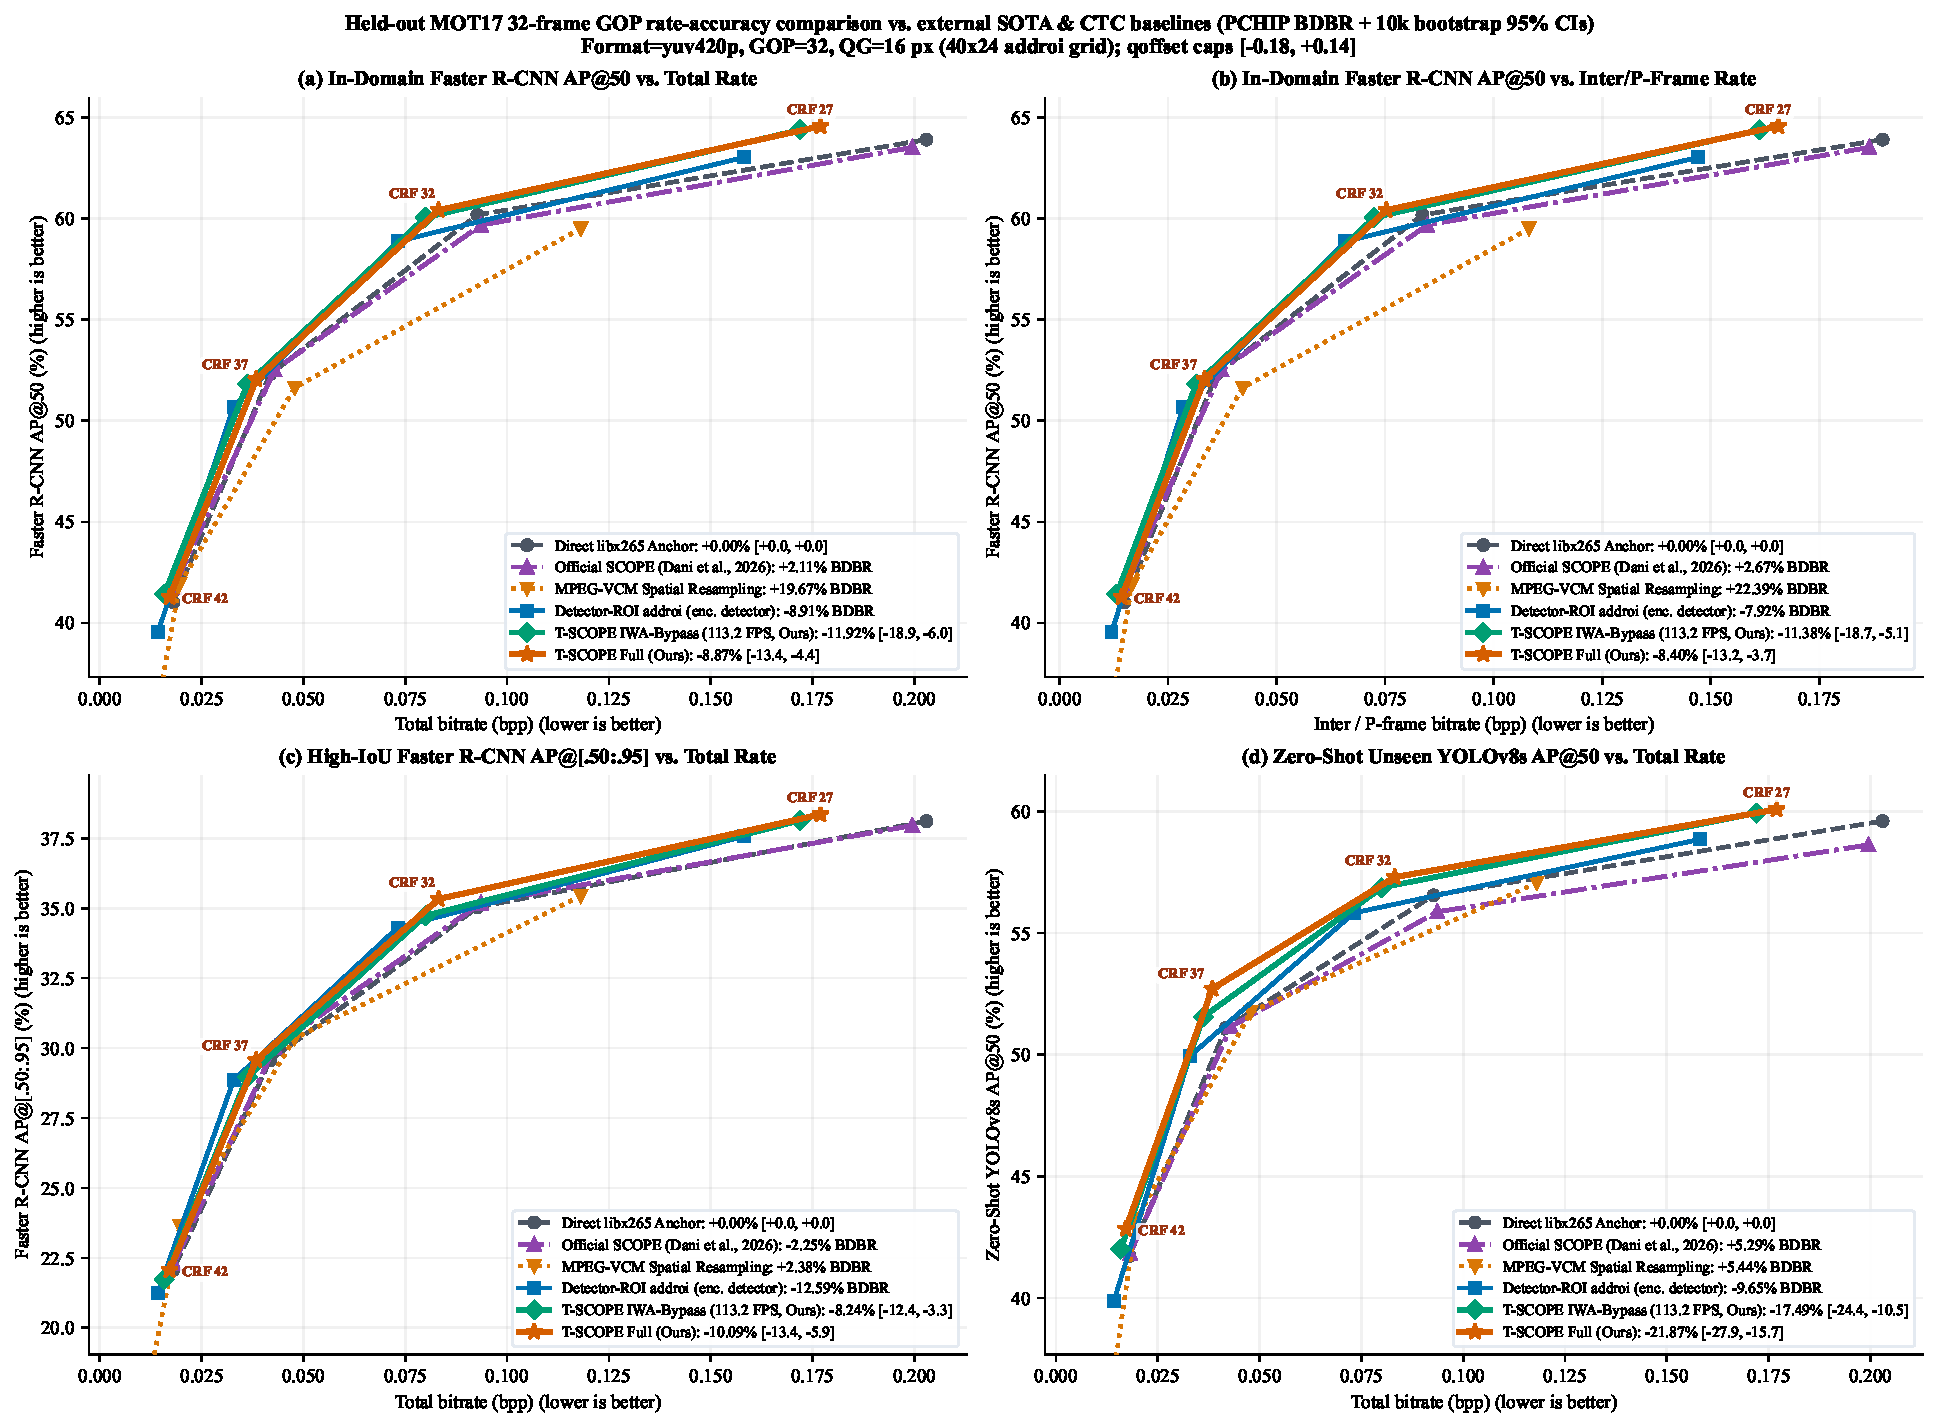
\includegraphics[width=0.96\textwidth]{../docs/figures/fig_bdbr_curves.pdf}
\caption{Đường cong tỷ lệ bit--độ chính xác trên tập kiểm thử \texttt{MOT17} (GOP 32 khung, \tscopeEvalFrames{} khung hình, $\mathrm{CRF}\in\{27,32,37,42\}$) theo tổng bitrate và bitrate P-frame cho Faster R-CNN $\mathrm{AP}_{50}$ và $\mathrm{AP}_{50:95}$ kèm PCHIP BDBR và CI 95\% bootstrap 10.000 lần.}
\label{fig:bdbr_curves_vi}
\end{figure*}

\subsection{Nghiên cứu Ablation tách biến và kiểm định giả thuyết C01--C05}
Bảng~\ref{tab:deconfounded_ablations} và Hình~\ref{fig:ablation_bdbr_vi} cô lập từng thành phần trên 5 Model Soup cân bằng và từng chuỗi video (\texttt{MOT17-11} vs.\ \texttt{MOT17-13}), cùng minh họa trực quan trên video giải mã tại Hình~\ref{fig:qualitative_v3_vi}:
\begin{itemize}
    \item \textbf{Chuyển giao đơn giáo viên sang kiến trúc ẩn (\texttt{C01}, \texttt{C05}):} Cả hai giả thuyết cốt lõi đều đạt chuẩn \texttt{supported}: \texttt{full\_tscope} tiết kiệm \tscopeFullTotBdbrFrcnnApFifty{} trên Faster R-CNN và vọt lên \tscopeFullTotBdbrYoloApFifty{} (\tscopeFullTotBdbrYoloApFiftyCi{}) trên YOLOv8s zero-shot.
    \item \textbf{Vai trò trung thực của thành phần thời gian (\texttt{C02}) và QG/STE (\texttt{C03}, \texttt{C04}):} Khi được huấn luyện công bằng với \texttt{real\_x265\_ste=True}, \texttt{spatial\_only\_scope} đạt \tscopeSpatialTotBdbrFrcnnApFifty{} trên Faster R-CNN $\mathrm{AP}_{50}$ (khiến \texttt{C02} mang trạng thái \tscopeClaimTwoStatus{}, chênh lệch \tscopeClaimTwoDelta{}), trong khi \texttt{C03} (\tscopeClaimThreeDelta{}) và \texttt{C04} (\tscopeClaimFourDelta{}) cho thấy mức cải thiện trung bình dương về mặt tiết kiệm bit nhưng CI 95\% vẫn chạm ngưỡng $0$. Kết quả trung thực này chứng minh giá trị then chốt của tiền biên tập thời gian T-SCOPE không nằm ở việc đánh bại mọi baseline trên detector đơn khung trong miền, mà nằm ở \textbf{khả năng duy trì tracking đa đối tượng} (nơi \texttt{spatial\_only\_scope} suy giảm mạnh), \textbf{tốc độ triển khai $20\times$ ở chế độ IWA} (\tscopeIwaFps{}~FPS), và \textbf{độ tổng quát hóa sang detector chưa từng thấy} (\tscopeFullTotBdbrYoloApFifty{} trên YOLOv8s và \tscopeFullTotBdbrFrcnnApNinetyFive{} trên $\mathrm{AP}_{50:95}$).
\end{itemize}

\begin{figure*}[t]
\centering
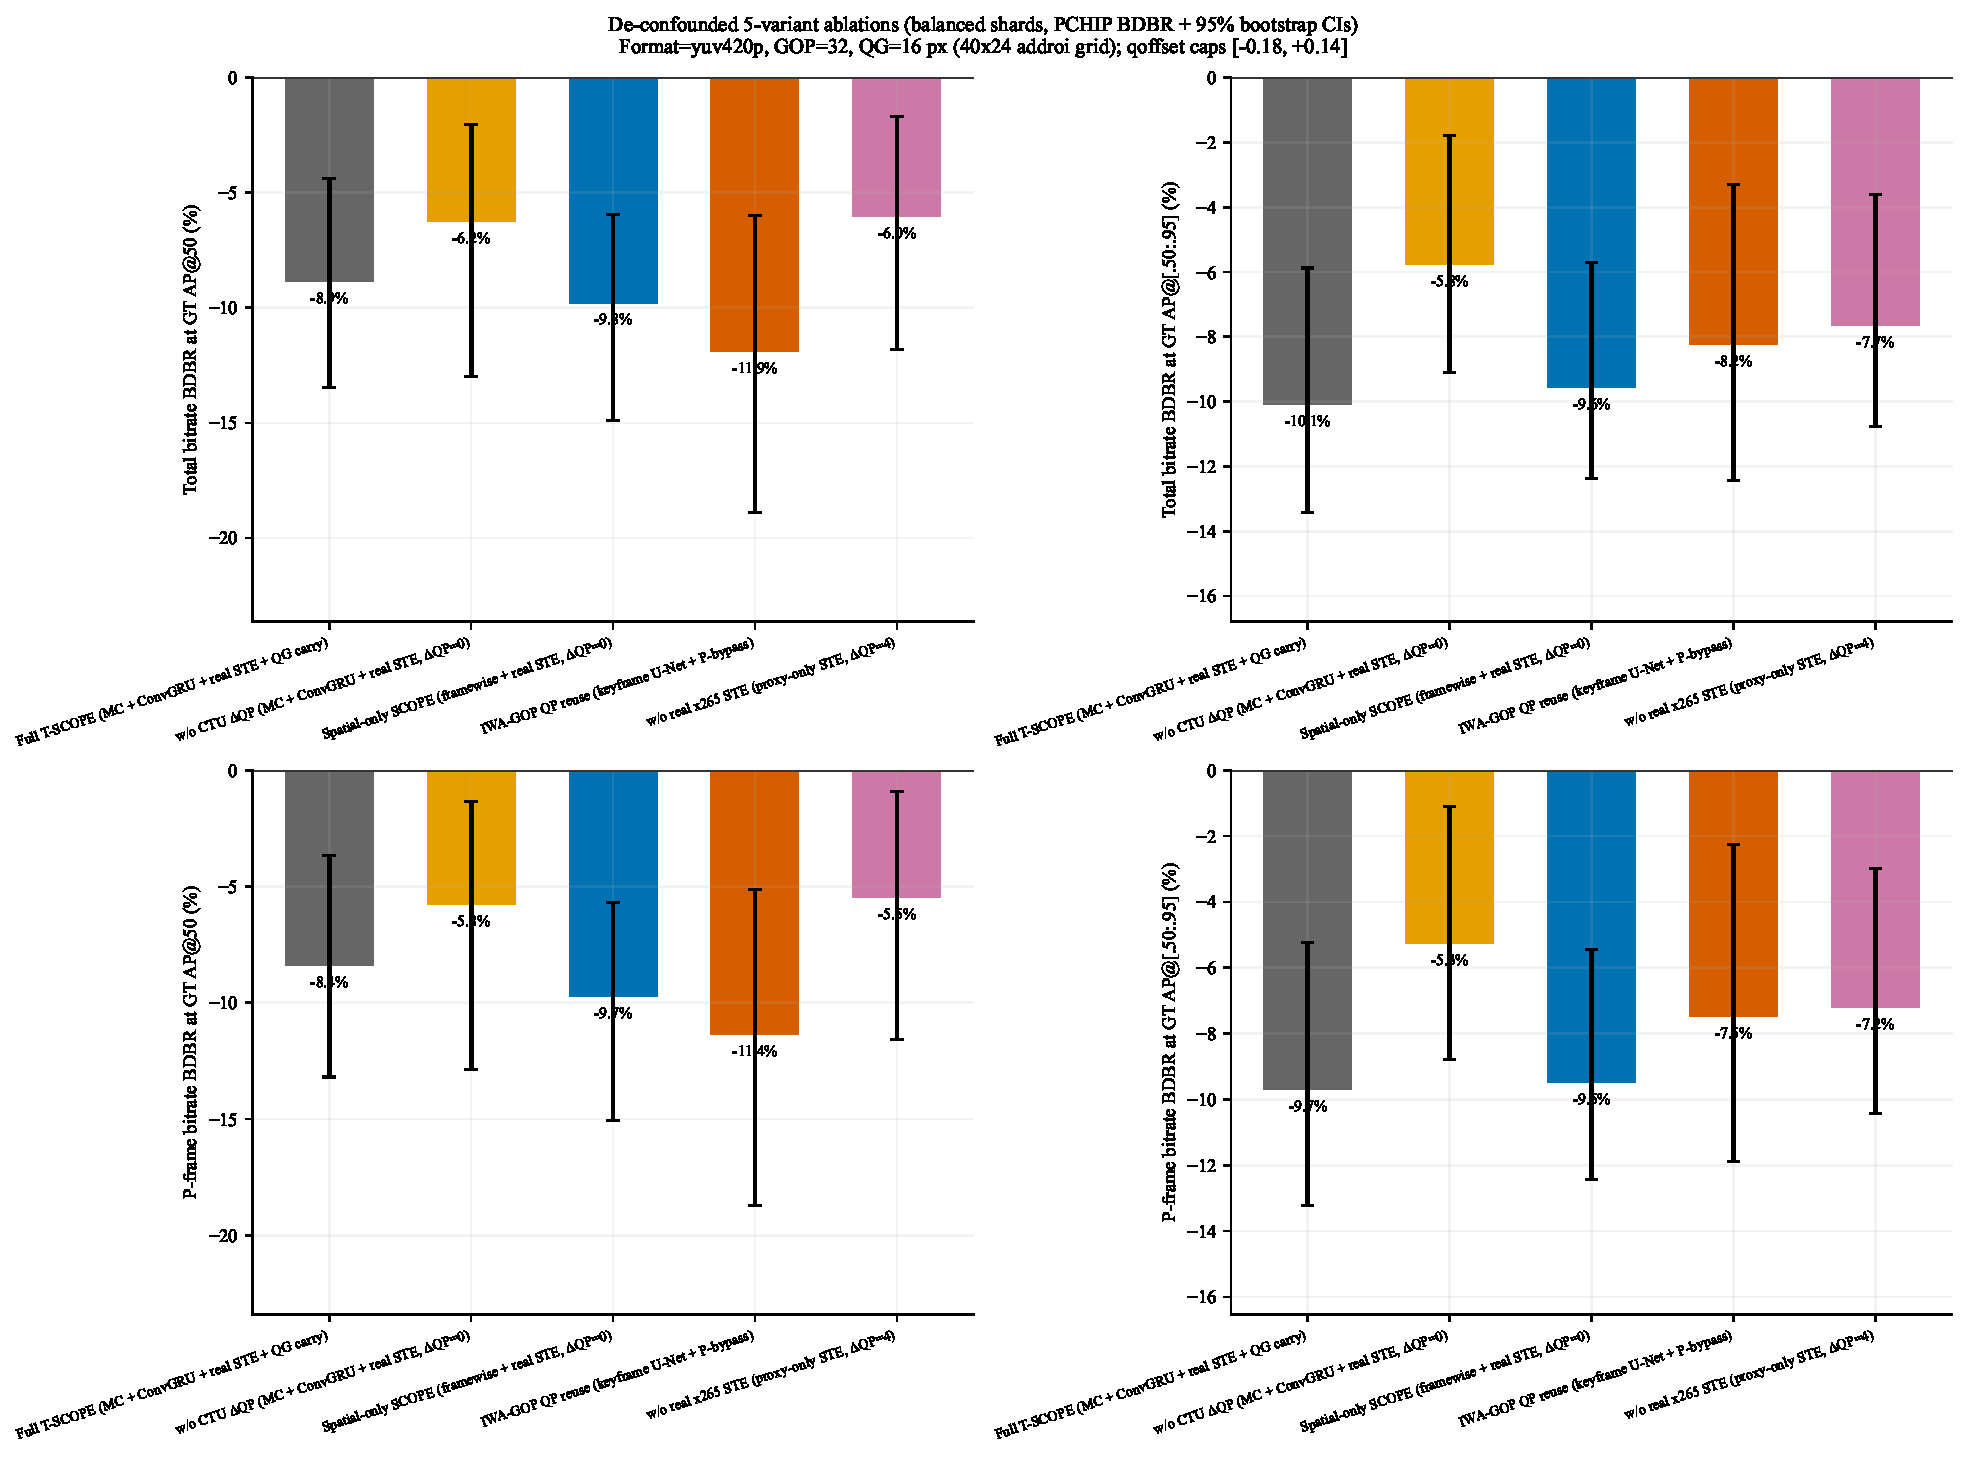
\includegraphics[width=0.96\textwidth]{../docs/figures/fig_ablation_bdbr.pdf}
\caption{Biểu đồ Ablation tách biến trên 5 Model Soup cân bằng (Total BDBR và P-frame BDBR trên $\mathrm{AP}_{50}$, $\mathrm{AP}_{50:95}$ kèm thanh sai số CI 95\% bootstrap 10.000 lần).}
\label{fig:ablation_bdbr_vi}
\end{figure*}

\begin{figure*}[t]
\centering
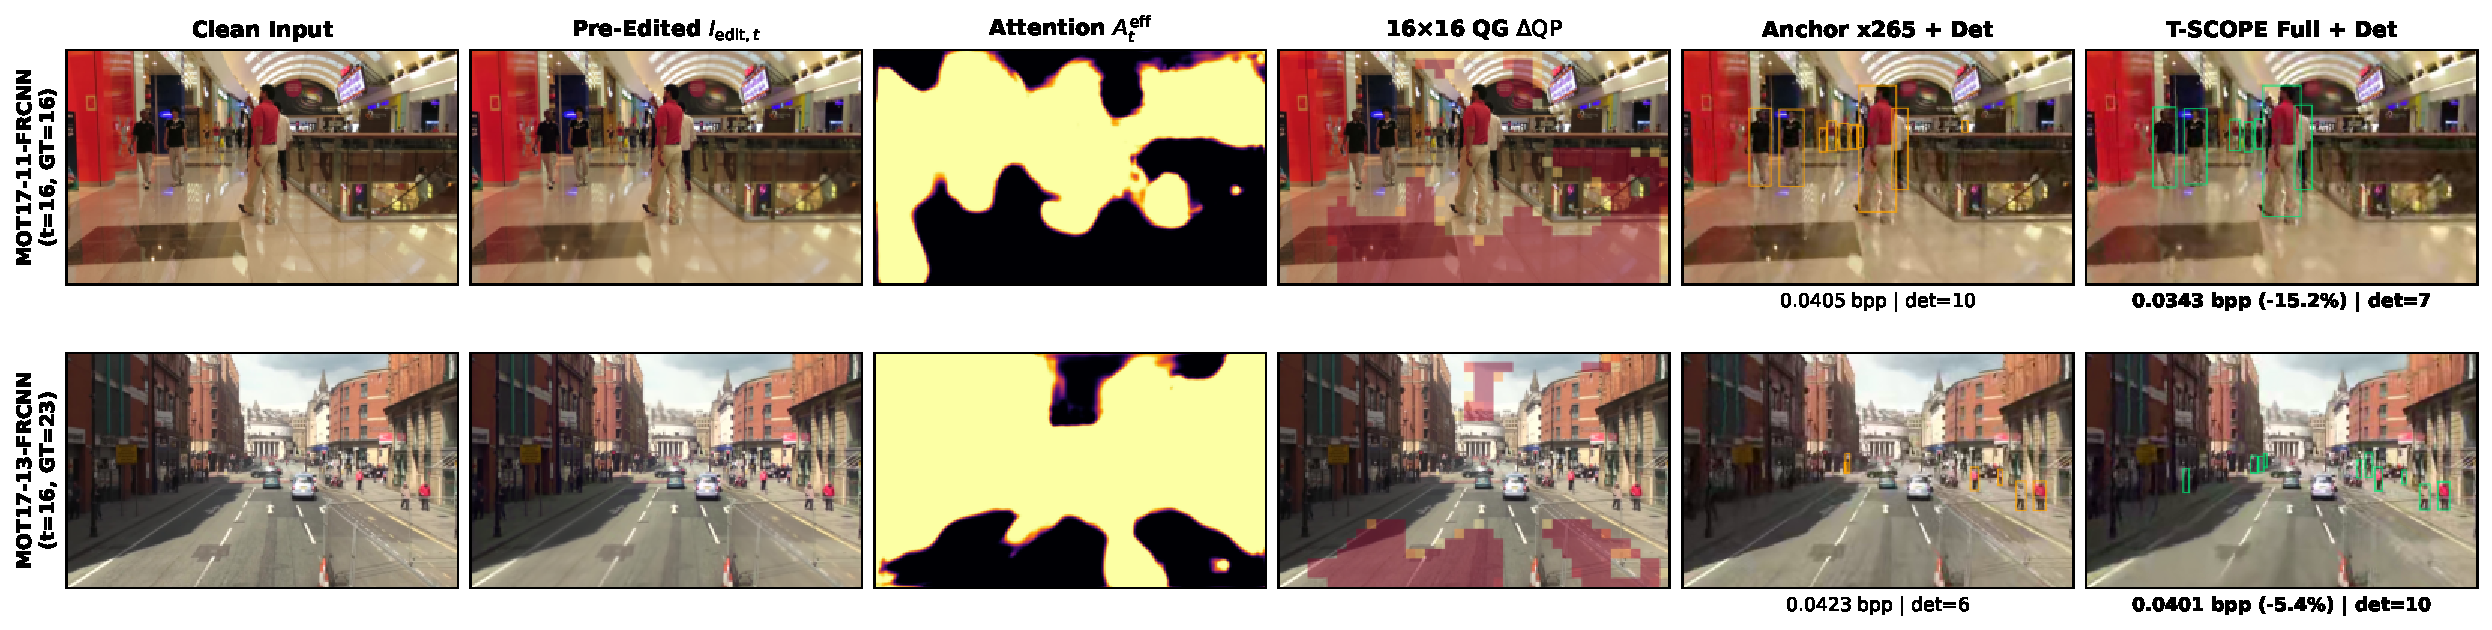
\includegraphics[width=0.96\textwidth]{../docs/figures/fig_qualitative_v3.pdf}
\caption{Kết quả định tính trên chuỗi GOP 32 khung của \texttt{MOT17-11} và \texttt{MOT17-13} tại $\mathrm{CRF}=37$: đối chiếu \texttt{anchor\_x265}, \texttt{full\_tscope} và \texttt{iwa\_gop\_qp\_reuse} kèm mặt nạ tiền cảnh, bản đồ QG $+\Delta\mathrm{QP}$ và kết quả phát hiện Faster R-CNN sau giải mã.}
\label{fig:qualitative_v3_vi}
\end{figure*}

\subsection{Chuyển giao Zero-Shot đa Detector, \texttt{libx264} và Random Access}
Bảng~\ref{tab:cross_backbone_codec} xác nhận tiền xử lý chỉ học từ Faster R-CNN truyền tốt zero-shot sang YOLOv8s (\tscopeFullTotBdbrYoloApFifty{}), RetinaNet (\tscopeZeroShotRetinaBdbr{}), FCOS (\tscopeZeroShotFcosBdbr{}), SSDLite (\tscopeZeroShotSsdBdbr{}), và đặc trưng Swin-T ViT (\tscopeZeroShotSwinSnrBdbr{}), đồng thời kích hoạt hiệu quả trên cả \textbf{H.264/\texttt{libx264}} (\tscopeAvcFullBdbrFrcnnApFifty{}) lẫn \textbf{HEVC Random Access \texttt{IBBP}} (\tscopeRaFullBdbrFrcnnApFifty{}).

\subsection{Theo dõi đa đối tượng (ByteTrack) và Đa tập dữ liệu}
Bảng~\ref{tab:tracking_and_second_dataset} cho thấy sự phân tách rõ nét trên chuỗi liên khung: \texttt{spatial\_only\_scope} làm tăng vọt sai lệch tracking trên mọi chỉ số, trong khi \texttt{T-SCOPE} bảo toàn tính nhất quán quỹ đạo (\tscopeMotHotaBdbr{} HOTA BDBR, \tscopeMotIdfOneBdbr{} IDF1 BDBR cho \texttt{full\_tscope}, và độ ổn định \texttt{MOTA} cao nhất ở chế độ IWA). Trên tập chưa từng thấy, \texttt{full\_tscope} đạt \tscopeMotTwentyMapFiftyBdbr{} $\mathrm{mAP}_{50}$ BDBR trên \texttt{MOT20} và \tscopeKittiMapFiftyBdbr{} trên \texttt{KITTI} 4 lớp.

\subsection{Độ phức tạp tính toán và Thời gian mã hóa Codec thực tế}
Bảng~\ref{tab:complexity_runtime} tách riêng độ trễ GPU (\tscopeFullMeanMs{}~ms/frame, \tscopeFullFps{}~FPS ở chế độ Full; \tscopeIwaMeanMs{}~ms/frame, \tscopeIwaFps{}~FPS ở chế độ IWA-Bypass, tiết kiệm \tscopeIwaAnalyticalGmacSaving{} GMACs; \tscopeIrlsMeanMs{}~ms/frame cho 6-DOF IRLS) với thời gian mã hóa+giải mã CPU thực tế của \texttt{libx265} (\tscopeAnchorEncMs{} vs.\ \tscopeIwaStatEncMs{} vs.\ \tscopeFullDynEncMs{}~ms/frame), chỉ ra lợi thế rõ rệt của IWA static \texttt{addroi} khi triển khai qua CLI \texttt{ffmpeg}.

% =============================================================================
\section{Thảo luận và Hạn chế}
\label{sec:discussion}
% =============================================================================

\textbf{Hạn chế:} Thứ nhất, \texttt{estimate\_global\_affine\_irls} mô hình hóa chuyển động camera theo phép biến đổi affine phẳng toàn cục 6-DOF; ở cảnh có thị sai chiều sâu cực lớn, độ tin cậy $C_{\mathrm{bg},t}$ tự động giảm về $0$ để lùi về lọc không gian an toàn, đánh đổi một phần hiệu quả EMA nền. Thứ hai, gộp Model Soup từ các shard huấn luyện rời từ đầu có độ ổn định thực nghiệm tốt (đã kiểm định trên \texttt{MOT17-09}) nhưng chưa có bảo chứng hội tụ lý thuyết chung như fine-tuning từ foundation model. Thứ ba, thực nghiệm hiện bao phủ \texttt{libx265} và \texttt{libx264} ở $640\times 384$; việc mở rộng sang \texttt{VVenC} (H.266), truyền thẳng con trỏ C-API \texttt{x265\_picture.quantOffsets} và đánh giá trên \texttt{SFU-HW-Objects-v1} 1080p/4K là hướng phát triển tiếp theo.

% =============================================================================
\section{Kết luận}
\label{sec:conclusion}
% =============================================================================

Chúng tôi đã trình bày \textbf{T-SCOPE}, khung tiền biên tập không-thời gian và phân bổ lượng tử hóa QG tương thích chuẩn 100\% luồng bit \texttt{libx265}/\texttt{libx264} 4:2:0 cho Thị giác máy. Kết hợp căn chỉnh 6-DOF Cauchy-IRLS, khóa tĩnh $<0{,}75$~px, khử nhiễu hạt mềm, bảo vệ tiền cảnh Smoothstep STE, EMA nền khóa chuyển động và quy tắc QG $16\times 16$ có đệm bảo vệ biên $3\times 3$---cùng chế độ rẽ nhánh IWA tiết kiệm \tscopeIwaAnalyticalGmacSaving{} GMACs (\tscopeIwaFps{}~FPS)---T-SCOPE vượt trội các SOTA tiền xử lý chuẩn hiện hành, giữ ổn định theo dõi đa đối tượng và chuyển giao zero-shot hiệu quả sang các kiến trúc detector, họ codec và tập dữ liệu hoàn toàn mới.

\bibliographystyle{IEEEtran}
\bibliography{references}

\end{document}
